\documentclass[12pt,twocolumn]{article}

\usepackage{fullpage}
\usepackage{graphicx}
\usepackage{graphics}
\usepackage{subfigure}
\usepackage{mdwlist}
\usepackage{floatrow}
\usepackage{blindtext}
\usepackage{algorithm2e}
\usepackage{algpseudocode}
\usepackage{pifont}
\usepackage{multirow}
\usepackage{floatrow}
\usepackage[toc,page]{appendix}


% christos: these look closer to NSF specs\dots
\setlength{\oddsidemargin}{0.0in}
\setlength{\evensidemargin}{0.0in}
\setlength{\textwidth}{6.5in}
\setlength{\headheight}{0.0in}
\setlength{\topmargin}{0.0in}
% \setlength{\textheight}{9.0in}
\setlength{\textheight}{9in}
\addtolength{\textheight}{-\topmargin}
\addtolength{\textheight}{-\headheight}
\addtolength{\textheight}{-\headsep}
\addtolength{\textheight}{-\footskip}


%\DeclareCaptionFont{Small}{\fontsize{6}{8}\selectfont}
%\DeclareFloatFont{normal}{\normalsize}
%\floatsetup{font={Small},heightadjust=object}

\begin{document}
\newfloatcommand{capbtabbox}{table}[][\FBwidth]
\newcommand{\beq}{\begin{equation}}
\newcommand{\eeq}{\end{equation}}
\newcommand{\bit}{\begin{itemize*}}
\newcommand{\eit}{\end{itemize*}}
\newcommand{\goal}[1]{ {\noindent {$\Rightarrow$} \em {#1} } }
\newcommand{\hide}[1]{}
\newcommand{\comment}[1]{ {\footnotesize {#1} } }
\newtheorem{lemma}{Lemma}
\newtheorem{theorem}{Theorem}
\newtheorem{proof}{Proof}
\newtheorem{defn}{Definition}
\newtheorem{algo}{Algorithm}
\newtheorem{observation}{Observation}

\title{Beyond Trigram: Learning to Distinguish Fake Article\\11-761 Project Report}


\author{ 
	{\em Yanran Hao} \\
	    {\tt yanranh@andrew.cmu.edu}
	 \and
	 {\em Yulan Huang} \\
	    {\tt yulanh@andrew.cmu.edu}
	  \and  
	{\em Ang Lu} \\
	    {\tt alu1@andrew.cmu.edu}
	 \and
	 {\em Heqing Ya} \\
	     {\tt heqingy@andrew.cmu.edu}
        }


\maketitle
%\begin{abstract}
%    \input{000abstract}
%\end{abstract}

\section{Introduction}
    \label{sec:intro}
    With the development of Language Technology, people have construct models to formally describe the natural language we are using in daily life.
Interestingly, some of the models have been powerful enough to generate fake articles that could even mix the false with the genuine.
Three MIT students developed a program called SCIgen\footnote{website: https://pdos.csail.mit.edu/archive/scigen/} that can automatically
generate an SCI article. They eventually fooled reviewers in several IEEE conferences with the generated articles. Therefore, a challenge is before
us: how can we tell the machine generated articles from human written ones. Finding such methods will not only avoid being fooled, but
can also help us build more powerful language model to make fun of the incompetent paper reviewers. 

In this project, we have extracted several features, and built several classification models to distinguish the fake generated by tri-gram models and 
 true articles. According to our experiment result , we have reached about 90\% accuracy in cross validation and development set. 

\section{Feature Generation}
    \label{sec:feature}
    \subsection{Semantic Feature}
For semantic features, we've explored features related to content/stop words and the features about word pairs.\\\\
%\begin{enumerate}
%  \item Features about content/stop words.\\
%\\Stop words are word which are filtered out before or after processing of natural language data. We use a stop words list 98 common stop words.\\
%\\Content words are words such as nouns, most verbs, adjectives, and adverbs that refer to some object, action, or characteristic. We generate a content word list using the training data according to words? frequency. We retrieved the words ranks top (using a threshold) and removed stop words.\\
%    \item Feature about word pairs
%\end{enumerate}
\textbf{1. Features about content/stop words} 
\\\\Stop words are word which are filtered out before or after processing of natural language data. We use a stop words list 98 common stop words.\\
\\Content words are words such as nouns, most verbs, adjectives, and adverbs that refer to some object, action, or characteristic. We generate a content word list using the training data according to words? frequency. We retrieved the words ranks top (using a threshold) and removed stop words.\\\\
\textbf{2. Feature about word pairs}
\\\\We use Yule's measure of association as measuring the correlation between word pairs.[1] The measure of semantic association will be defined based on the contingency table below.
\begin{figure}[!h]
\centering  
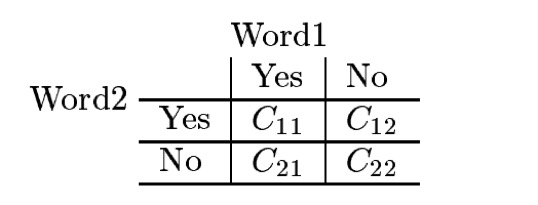
\includegraphics[width = 0.7\linewidth]{./FIG/030/contigency}\hfill
\label{fig:020feature}
\end{figure}
For each word pair, $C_{11}$ is the count of sentences in the training corpus that contains the word pair; $C_{12}$ is the 
subtraction of the count of sentences contains word1 and $C_{11}$; $C_{21}$ is the subtraction of the count of sentences contains word2 and $C_{11}$; $C_{22}$ is the total number of sentences subtracting $C_{11}$, $C_{12}$ and $C_{21}$.\\
\\Then we calculate the Q-statistics as the correlation value between word pairs:
\begin{equation}
	Q=\frac{C_{11}C_{22} - C_{12}C_{21}}{C_{11}C_{22} + C_{12}C_{21}}
\end{equation}
The higher value of Q, the stronger the correlation between the two words.\\\\
Based on the above two categories, we designed our features as:
\vspace{-\topsep}
\begin{itemize}
  \setlength{\itemsep}{4pt}
    \setlength{\parskip}{0pt}
%    \setlength{\parsep}{0pt}  
  \item The ratio of stop words and content words.
  \item The general statistics of correlation value of word pairs.\\[5pt]
We calculate the mean, variance, maximum, minimum, mean and range of the correlation value of word pairs. Moreover, we created a subgroup of words pairs that only contains distant word pairs (distance  $\geq$5) and calculated the above feature for this group too.
 \item Percentage of high correlation values.\\[5pt]
This features detects the percentage of pairs that have high correlation values. We use a threshold to determine what is the standard of high.
 \item Percentage of unseen pairs.\\[5pt]
Real articles would have a relative stable percentage of unseen pairs while fake articles will have either too high or too low percentage. We believe that this feature can help us distinguish between real and fake.
 \item Repetition of phrases.\\[5pt]
Similar to the previous one, real articles would have a relative stable percentage of phrases repetitions while fake articles will have either too much repetition or little repetitions. We calculate the percentage of repetitions and the length of longest repeated phrases (single words are treated as special phrases too).
 \item Coherence score.\\[5pt]
Coherence score are defined as the average correlation value of distant (distance $\geq$5) content pairs.
 \item Latent Semantic Analysis (LSA).\\[5pt]
Inspired by the indexing technology, we've applied the idea of LSA to create a new feature which we believe can help improving the classification performance.[2] Let $X_{m\times{n}}$ be a matrix where element $X_{ij}$ describes the frequency of $Word_{i}$ in $Sentence_{j}$. Now, the dot product of $A_{n\times{n}} = X^{T}X$ contains all the dot products between the word vectors gives the correlation between the term over sentences. By using singular value decomposition (SVD), we can get  \begin{equation}
	A = U\Sigma{V^T}	
\end{equation}
Here, $\Sigma_{n\times{n}}$ is the diagonal matrix contains the singular value. Based on LSA, when you select the top $k$ largest singular values and their corresponding singular vectors from $U$ and $V$, you get the approximation to $A$. We use a threshold to select the top $k$ singular values and calculate the $A_{k}$. We use
\begin{equation}
	loss = \|A - A_{k}\|
\end{equation}
as the feature which represent the information loss using approximation. For real articles, the loss should be small while fake articles should be relatively large.

 
\end{itemize}


\subsection{Syntactic Feature}
Based on the hypothesis that trigram model cannot capture the syntactic features of sentence and the fake sentence are less grammatical, we measures the grammaticality of a sentence and uses it as one of our feature. More precisely, we parsed both real and fake sentences in the training data using the Charniak Parser in NLTK and got the likelihood of the highest ranked parsing tree for each sentence. We derived the overall grammaticality score by 
$$P_{Gram} = \frac{\sum_{i=1}^N L_iP(S_i)}{\sum_{i=1}^N L_i}$$
However, the syntactic feature is only able to improve the prediction a little bit in the training set and is very time-consuming. Thus, we abandoned it to be further used in the test set.
The potential reason for the syntactic feature to be such useless might be that our data contains spoken scripts, which are much less grammatical than the official written language. Another reason might be that the parser is not accurate, since it was trained in mixcase corpus, while our corpus was all uppercase.

\subsection{Statistical Feature}
We also defines some statistical features for the data.

\begin{itemize}
\item Ratio of perplexity of trigram and quad-gram models

Since the trigram model cannot capture information in the quad-gram model, we uses the ratio of perplexity of trigram and quad-gram models as one of the features. Since our training data is very small, the variance of the estimation will be very big. Thus, we used the same BNC corpus to estimate the probabilities of both trigram and quad-gram models. While the two type of articles will both have low perplexity score for the tri-gram model, the real articles would have lower perplexity for the quad-gram model than the fake articles. This implies that the ratio of trigram to quad-gram perplexities would be lower for a fake article than for a real article. Figure \ref{fig:ratio} shows the distribution of the feature in real articles and fake articles in the training data. As we can see, there is a significant difference of the feature between real and fake articles, which indicates that this is a good feature for distinguish two types of articles. 

\item Count of uncommon pairs of words
Content words are frequently occurring words in corpus that are not stop words. We ranked all words in the training data using their frequency and uses rank between 150 to 6500 word types as the content words. We then define the common content word pairs as content words that are at least 5 words apart in the real documents and are having frequency above some threshold. For a given article, a list of content word pairs is compared against this list and word pairs not in this list form the set of uncommon word pairs. 

We assume that a real article is expected to have lesser number of uncommon content-word pairs than fake articles. So we used probability of finding an uncommon content-word pair in an article as one of our features. This probability is greater for fake articles than the real articles and we use this probability as a feature for the classification task.
\end{itemize}

\begin{figure}
\centering  
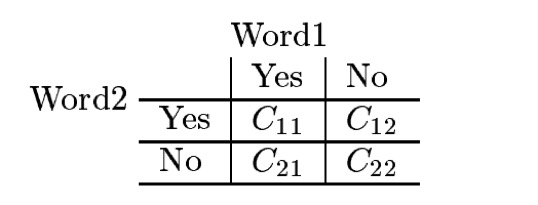
\includegraphics[width = \linewidth]{./FIG/030/ratio}\hfill
\caption{Histogram for the ratio of perplexity of trigram and quadgram} \label{fig:ratio}
\end{figure}



    
%\vspace{3cm}
%\section{Proposed Method}
%    \label{sec:proposed}
%   \input{030method}


\section{Experiments}
    \label{sec:experiments}
    \subsection{Data Description}
The training set is 1000 articles, 500 real and 500 fake, of varying length. The development set is 200 articles, 100 fake, 100 real. Articles in development set is truncated to meet the length distribution in Table ~\ref{tab:040dev}. Besides these two sets, we also use a 100 million word corpus of Broadcast News articles as external source for generation of specific feature.
\begin{table}
	\begin{center}
		\begin{tabular}{|c|c|}
		\hline
		\#sentence&\#article\\
		\hline
		1&20\\
		2&10\\
		3&10\\
		4&10\\
		5&10\\
		7&10\\
		10&10\\
		15&10\\
		20&10\\
		\hline
		\end{tabular}
	\end{center}
	\label{tab:040dev}
	\caption{Article length distribution of dev set}
\end{table}
\subsection{Data Preprocessing}
Articles from training set are truncated following the document length distribution in Table ~\ref{tab:040dev}. The number of truncated training articles is 10065. Sentence per article distributions of original training set, truncated training set and development set are shown in Figure ~\ref{fig:040length}.

\begin{figure*}
\centering  
\subfigure[Training set (original)]{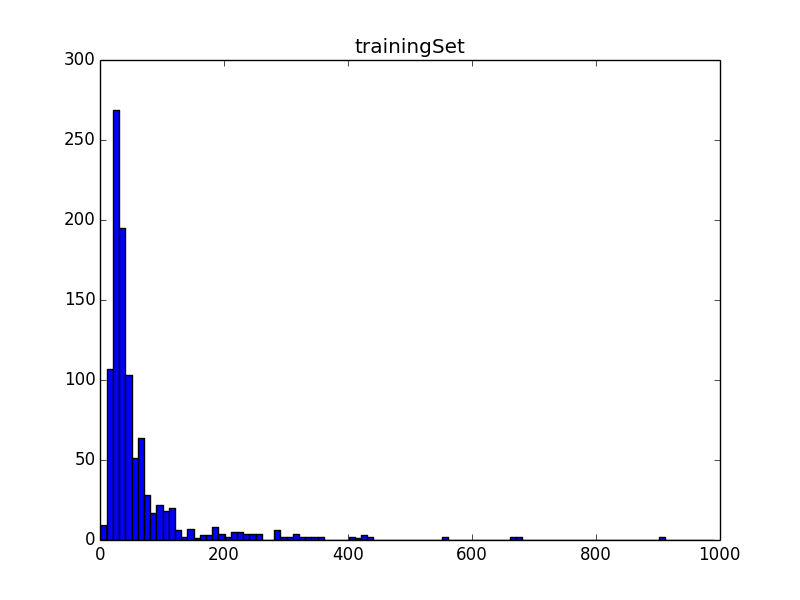
\includegraphics[width=0.33\linewidth]{./FIG/040/trainingdist.png}}\hfill
\subfigure[Training set (truncated)]{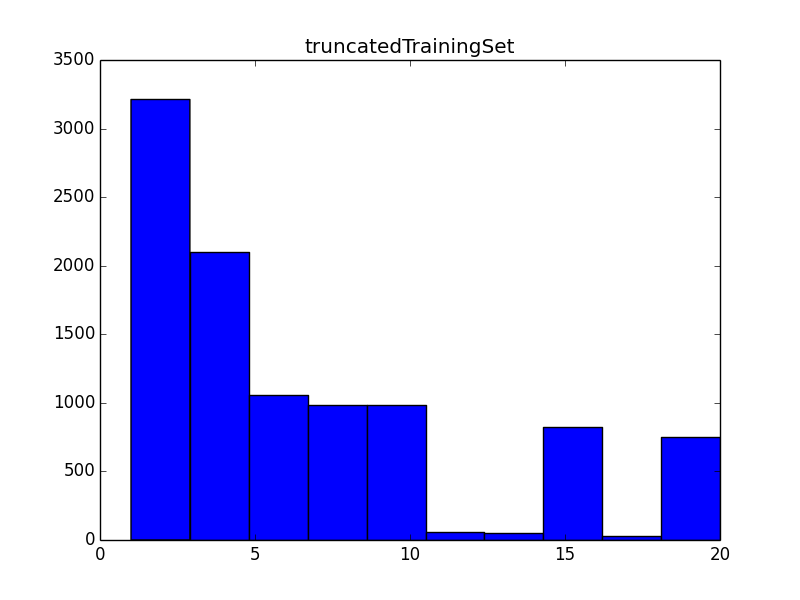
\includegraphics[width=0.33\linewidth]{./FIG/040/trunceddist.png}}\hfill
\subfigure[Dev set]{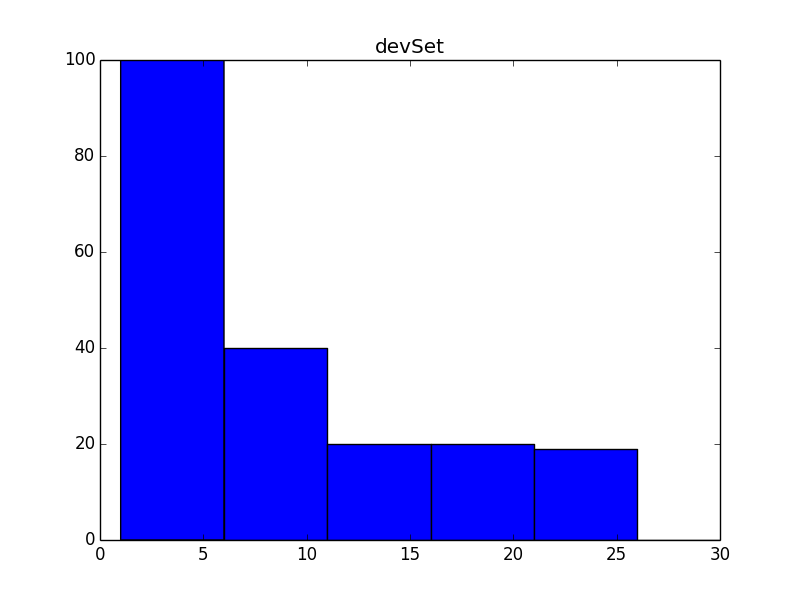
\includegraphics[width=0.33\linewidth]{./FIG/040/devdist.png}}\\

\caption{Article length distribution of different sets}
\label{fig:040length}
\end{figure*}

\subsection{Classifier Choice}
Popular classifiers for binary classification task are chosen as candidates, including KNN, logistic regression, SVM, gradient boosting (xgboost). Testing individual feature on development set and cross validation on training set, xgboost outperforms all the other algorithm by about 5\%. Also it is very fast comparing to SVM. So we choose xgboost as the final classier.

\subsection{Results}
The results of different feature sets are shown in Table ~\ref{tab:040res}. From the table we can tell that the statistical feature contribute most to the accuracy. Using it along could gave us a result close to the combined features. Syntactic features are not very useful in this experiment\footnote{Didn't run on dev set because of low performance on training set and large computation}. Although most semantic features fail to surpass an accuracy of 70, the combined semantic features get an accuracy of 80.
\begin{table}[!h]
	\begin{center}
		\begin{tabular}{|c|c|c|c|}
		\hline
		Features&Avg. cv Train&Dev&Soft\\
		\hline
		Semantic & 80.2 & 80.0 & 74.9\\
		Syntactic & 52.3 & &\\
		Statistical & 85.4 &88.0&81.7\\
		All combined & 89.4 & 89.0&86.0\\
		\hline
		\end{tabular}
	\end{center}
	\label{tab:040res}
	\caption{Experiment results}
\end{table}

\section{Conclusions}
    \label{sec:conclusions}
    In this project, we tackled the problem to distinguish real and fake documents, where the fake documents are generated based on a trigram model. we experimented three types of features, semantic feature, syntactic feature and statistical feature. We also built four classifiers, KNN, logistic regression, SVM and gradient boosting. In our experiment, we found that the statistical features is very useful when the statistics are estimated by MLE from large corpus, while has little use when the statistics is from small dataset. The semantic feature is also very useful even within small dataset. The syntactic features has less use in our experiment due to the lack of grammatical structure in spoken language. For classifiers, gradient boosting outperforms the other classifiers, since it is able to adapt different features we extracted to different documents. 
    
\clearpage
\bibliography{BIB/YLH,BIB/YRH,BIB/AL,BIB/HQY}
\bibliographystyle{plain}

\begin{appendices}
\section{Contribution}
    \label{sec:contribution}
    \begin{itemize}
\item Yanran Hao: Feature Implementation
\item Yulan Huang: Feature Implementation
\item Ang Lu: Classification Model Tuning
\item Heqing Ya: Data Pre-Processing, Codebase Implementation
\end{itemize}
\section{Comments}
    \label{sec:comments}
    This assignment gives us a chance to apply statistical method on classification problem, which is good practice 
for real problems that we will meet in the future. We analyzed the task together, and discussed what features
are reasonable, what models are best for this 2-class classification problem, and how we could develop the 
program together. 

We not only get a sense of how the language models work, but also learned techniques in
team management\footnote{We used team management tool Teambition to share files and manage tasks} 
and software engineering\footnote{We used Git for version control and Tmux to extract data and train model
remotely on server clusters, and parallelize our programs to accelerate the calculation}.

One thing that worth mentioning is that, for the 4-gram perplexity feature, which has the best performance among
all of ours, was almost 
\end{appendices}

%\newpage
%\appendix
%\section{Appendix}
%\input{099appendix}

%\newpage
%\pagenumbering{roman}
%\tableofcontents


\end{document}
